

\par In order to achieve the ability to predict objects and scenes 
from FMRI images, a predictive model is required. The project was thus 
divided into a few main stages for independent preprocessing of the 
movie description and FMRI images, model building, and prediction
testing.

\centerline{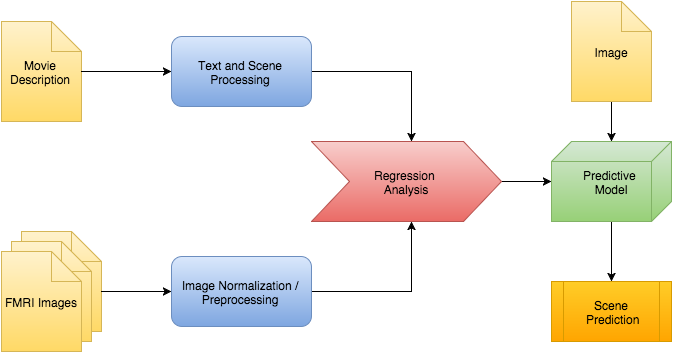
\includegraphics[width=.9\linewidth]{processflow}}

\subsection{Text Preprocessing}
\par As the movie description as provided was in German, we first used Google
Translate to translate the description to English before proceeding with 
any further processing. Though there may be translational errors, it was decided
that it was best to transform the original descriptions (versus using other english descriptions) to maintain the original timestamps from the researchers
to have optimal alignment between the description and FMRI data.

\par Due to grammatical differences, we decided to
 only keep nouns and verbs, and discarded the adjectives and other words including
 stopwords, which are commonly used words with little meaning or determinable context (e.g. 'and', 'to', 'him'). A publicly available list of stopwords from Princeton University was used for this task. 

 \par Of the words that remained, a WordNet dictionary was built, which is a 
 popular way to tag words according to a context-specific definition. In this way,
 words as stand-alone entitites will have an unambiguous definition and 
 deeper relationships can be derived from the correlations found. 

 \par After aggregating the set of all contextual definitions of words,
 we build a design matrix composed of the descriptive entries in the movie description.
 Thus each interval of time with a sentence description of the movie events was treated
 as a row, and each column represented a context-specific word as a feature. The matrix values are all binary, with a value of '1' indicating that the word is present in the sentence, while '0' indicates that it is not. This was illustrated as a rectangular image
 with a white square for '1' and black for '0'. 

 \centerline{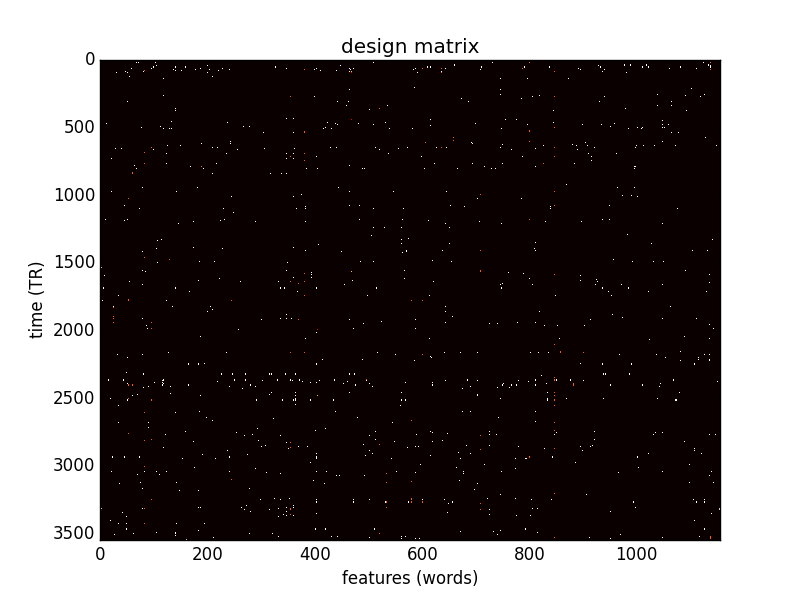
\includegraphics[width=.9\linewidth]{design_matrix}}

\par As can be seen, this matrix is relatively sparse.
\par Finally, in order to format the data such that it correlates explicitly
to the FMRI images, the intervals were split into two-second intervals
to create a one-to-one representation between description objects and images.


\subsection{FMRI Preprocessing}

\subsection{Regression Analysis}

\subsection{Predictive Testing}

